\documentclass[../rapport_MVEX01-11-05]{subfiles}
\begin{document}
\section{Statistisk klassificering}\label{sec:klassificering}

Klassificering är ett centralt statistiskt begrepp inom maskininlärning.
Det handlar om att klassificeraren ska göra en kvalificerad gissning för hur
observerad data ska hanteras, baserad på någon typ av ''inlärningsprocess''.
Man skiljer på modellbaserade och modellfria metoder, där de modellbaserade
bygger på modeller av de bakomliggande system som ska analyseras, medan de
modellfria kan ses som mer oberoende av sammanhang \cite{Hastie09}.
Man skiljer också på övervakad respektive icke-övervakad inlärning,
där man i det övervakade fallet har etiketter på den träningsdata man stoppar
in, så att man för varje objekt kan säga om det klassificerats rätt eller
fel.

Indata till klassificeraren är någon mängd av objekt med någon uppsättning
egenskaper (features) som kan mätas.
I egenskapsrummet önskar man då att objekten separeras i olika kluster
som stämmer överens med deras verkliga klass.
I vissa problem är resultatet binärt,
vilket exempelvis gäller i hudisoleringsproblemet.
I andra fall väljs bland många klasser, vilket gäller gestklassificeringen.
Svårigheten kan förtydligas något med hjälp av figur \vref{fig:kluster}.
\begin{figure}[!htpb]
    \begin{center}
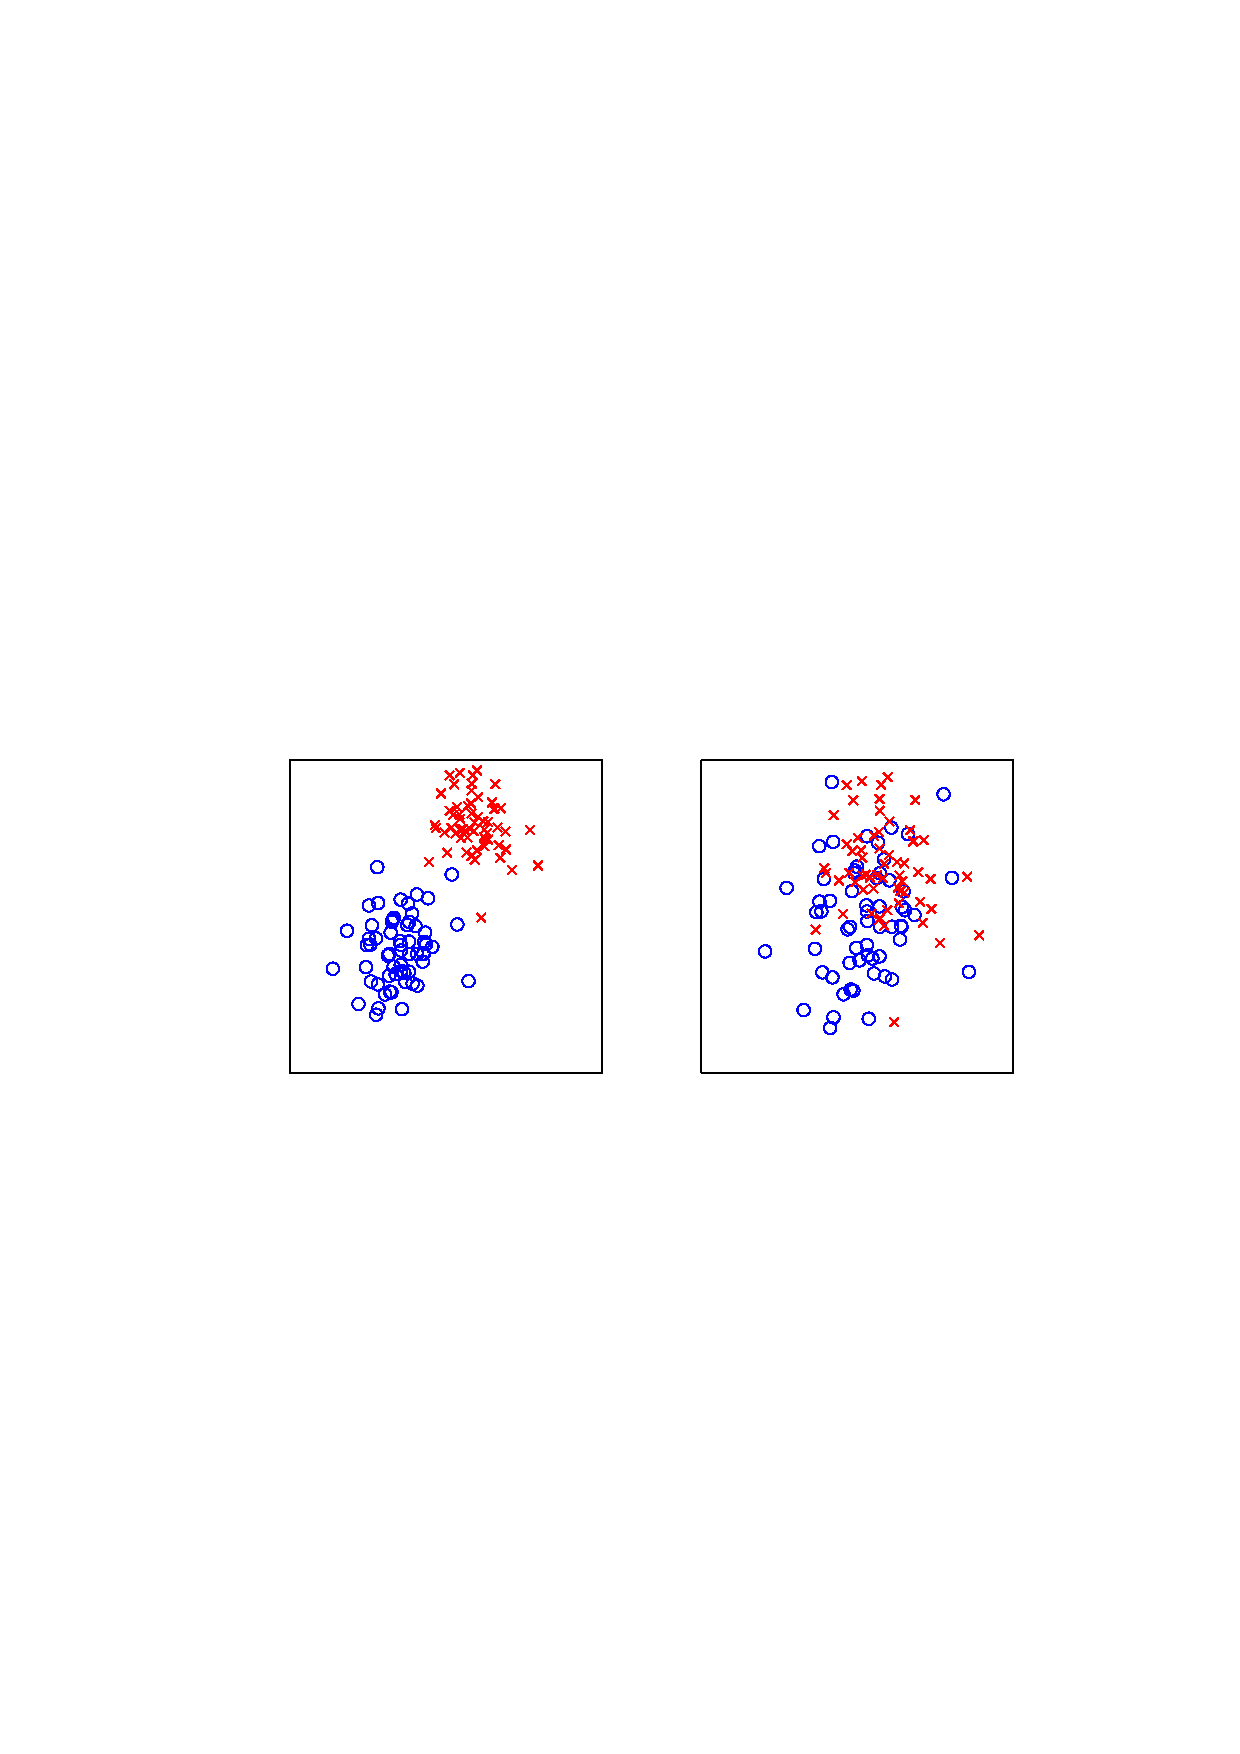
\includegraphics[width=0.8\textwidth,clip=true,trim=2cm 3cm 1.5cm 3cm]{bilder/kluster.pdf}
    \end{center}
    \caption{Det är enkelt att se var ett objekt hör hemma i den vänstra figuren,
    där de två klasserna är väl separerade. I den högra figuren kan man också se
    skillnad på objekt, men det är nu mycket svårt. Axlarna motsvarar
    två godtyckliga egenskaper. En annan uppsättning egenskaper kan ge en
    tydligare separering av klasserna.}
    \label{fig:kluster}
\end{figure}

Tre klassificerare kommer att beröras, den modellfria
prototypbaserade \knn samt de två modellbaserade Gaussian Mixture
Models och dolda Markovmodeller.

%Klassificering handlar om att göra en kvalificerad gissning
%i någon fråga, t.ex.~om en bildpunkt (pixel) innehåller hud, eller om ett område har
%en viss form. I denna mening måste man alltid ha ''träningsdata'' att jämföra med
%till sin
%klassificerare, även om det inte alltid handlar om faktisk träning. Angreppssätt
%så som dolda markovmodeller, random forests, genetiska metoder och liknande kräver
%träning i form av att känd data matas in i klassificeraren varpå denne
%konstruerar en struktur som används för framtida klassificering.
%Enklare metoder så som \knn 
%kräver endast känd data att jämföra med; denna data är då prototypdata.
%
%\notes{Behövs det mer här?}

\end{document} 

